\documentclass[10pt,a4paper]{article}
\usepackage[T1]{fontenc}
\usepackage{lmodern,textcomp}
\usepackage[margin=2.4cm]{geometry}
\usepackage{amsmath,amssymb,amsthm}
\usepackage{graphicx,booktabs,array,float}
\usepackage[hidelinks]{hyperref}
\usepackage{microtype}
\setlength{\parskip}{3pt}
\newtheorem{proposition}{Proposition}
\newtheorem{definition}{Definition}
\renewcommand{\arraystretch}{1.1}
\begin{document}
\title{\bfseries Remarketing Planner: Front-Loaded Email and SMS Calendars for Lead Lifetime Value\\[2pt]\large A six-month contact plan for consumer-finance leads}
\author{Humbert Pou Plana}
\date{November 2026}
\maketitle
\begin{abstract}
Remarketing to consumer-finance leads is usually run as a set of event-triggered emails with ad hoc timing. We propose a different design principle: spend the contact budget where response decays fastest, which is the first 24 hours, and then space contacts until the lead is considered inactive after 180 days. We formalise a simple response model with exponential decay, a fatigue penalty for recent contacts, channel-specific unsubscribe rates and an incrementality factor, and build a planner that produces a six-month email and SMS calendar for six lead segments derived from an event-based funnel. Under hypothetical but explicit parameters, the front-loaded calendar is never the worst of three calendars (it also beats a constant weekly email in three segments and an aggressive daily cadence in four), and it lifts lifetime value per lead from 11.00 to 11.98 euros in the main segment; the aggressive cadence earns slightly more in the two highest-value segments but at roughly double the unsubscribe rate, a cost the model does not price. Because every response parameter is a hypothesis, the paper's main output is a calendar and a validation design, not an effect size.
\end{abstract}

\section{Introduction}
Lifetime value (LTV) is the value a customer or lead generates over its life \cite{gupta}. For a lead generator, much of that value arrives after the first conversion: a lead who did not complete the application, was declined by every lender, or has a payment-default flag can still convert later through other products. The question is when to contact them and how often. Our operator's experience is that paid remarketing on advertising platforms performs poorly for this business because of low conversion, lower intent on second and third conversions and shorter LTV, and that a well-timed email and SMS flow with a small number of high-quality messages performs better. This paper formalises that approach.

\section{Funnel and segments}
The planner starts from an event-based funnel with the following entry points: a visitor who leaves before signing up; a first-step drop-off; a submitted application; an application declined by all lenders; a lead with a payment-default flag; a high-quality lead (stable income, working-age, permanent contract, no payment-default flag, consumer-credit amount in a defined range, home market only); and a cold list. Messages in the existing funnel are sent at fixed offsets after each event (for example 1 hour, 1 day, 3 days, 6 days after a first step; 1 hour, 2 days, 4 days after an application) and at long intervals thereafter. We retain those anchor times and reshape the rest of the calendar to concentrate contacts early and end at 180 days.

\section{Model}
A cohort of $N$ leads enters a flow at time $0$. Touch $k$ is sent at time $t_k$ days by channel $c_k\in\{\text{email},\text{SMS}\}$. Let $\alpha_k$ be the fraction of the cohort still active before touch $k$ (not converted, not unsubscribed). The model is
\begin{align}
 w(t)&=w_0+(1-w_0)e^{-t/\tau}, & \phi_k&=\frac{1}{1+\gamma\,m_k},\\
 \kappa_k&=\alpha_k\,r_{c_k}\,w(t_k)\,\phi_k, & u_k&=\alpha_k\,\mu_{c_k}\,(1+\eta\,m_k),\\
 \alpha_{k+1}&=\alpha_k-\kappa_k-u_k,
\end{align}
where $\kappa_k$ is the fraction converting at touch $k$, $u_k$ the fraction unsubscribing, $m_k$ the number of touches in the previous 48 hours, $r_c$ the base response of channel $c$, $\tau$ the segment's decay constant (days), $w_0=0.12$ the floor of the decay, $\gamma=0.3$ the fatigue parameter, $\mu_{\text{email}}=0.4\%$, $\mu_{\text{SMS}}=0.9\%$ the unsubscribe rates and $\eta=0.6$. Converted leads stop receiving touches. Incremental revenue is $\sum_k N\kappa_k\,V\,\iota$, with $V$ the value of a conversion and $\iota=0.7$ the incrementality (share of conversions that would not have happened anyway). Cost is $\sum_k N\alpha_k\,q_{c_k}$ with $q=0.003$ euros per email and $0.05$ euros per SMS. Net profit is revenue minus cost and the new LTV per lead is $L_0+\text{net}/N$.

\subsection{Design principle}
Because $w(t)$ decays and fatigue penalises bursts, the marginal value of a touch is highest soon after entry and falls quickly. A calendar that places many touches in the first 24 hours (SMS at 15 minutes, 3 hours and 12 hours; emails at 1 hour and 6 hours, and so on) captures the high-response window. After a week touches are spaced by several days and, after 55 days, by roughly one month, until a final notice and soft unsubscribe at day 180.

\section{Parameters}
Table~\ref{tab:par} gives the segment parameters. They are hypotheses chosen to be plausible and ordered sensibly (high-quality leads respond most, cold lists least); none is measured. Users of the planner can change every value.
\begin{table}[H]\centering\small\caption{Segment parameters: number of touches, base response per send for email / SMS (\%), decay constant $\tau$ (days), conversion value $V$ and baseline LTV $L_0$ (euros).}\label{tab:par}
\begin{tabular}{lrrrrr}\toprule Segment & Touches & Response (\%) & $\tau$ & $V$ & $L_0$\\\midrule
Application submitted & 21 & 1.8 / 3.0 & 6 & 14 & 11\\
First-step drop-off & 20 & 2.5 / 4.0 & 3 & 12 & 6\\
Declined by all lenders & 15 & 0.8 / 1.2 & 20 & 6 & 2\\
Payment-default flag & 15 & 1.0 / 1.5 & 10 & 8 & 3\\
High-quality lead & 18 & 3.0 / 4.5 & 8 & 22 & 18\\
Cold base & 16 & 0.4 / 0.6 & 60 & 10 & 1\\
\bottomrule\end{tabular}\end{table}

\section{Results}
\subsection{The calendar}
Figure~\ref{fig:tl} shows the calendar for the main segment: 21 touches, of which 6 in the first 24 hours; Figure~\ref{fig:bk} shows touches per period.
\begin{figure}[H]\centering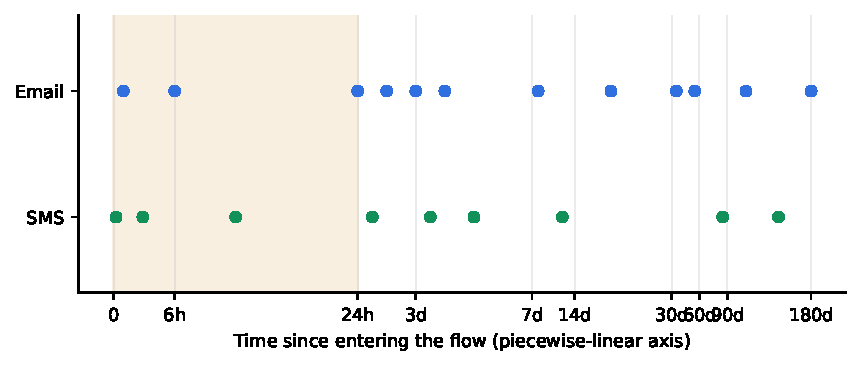
\includegraphics[width=0.92\linewidth]{fig/p3_timeline.pdf}\caption{Calendar for the main segment. Shaded area: first 24 hours; the time axis is piecewise linear.}\label{fig:tl}\end{figure}

\begin{figure}[H]\centering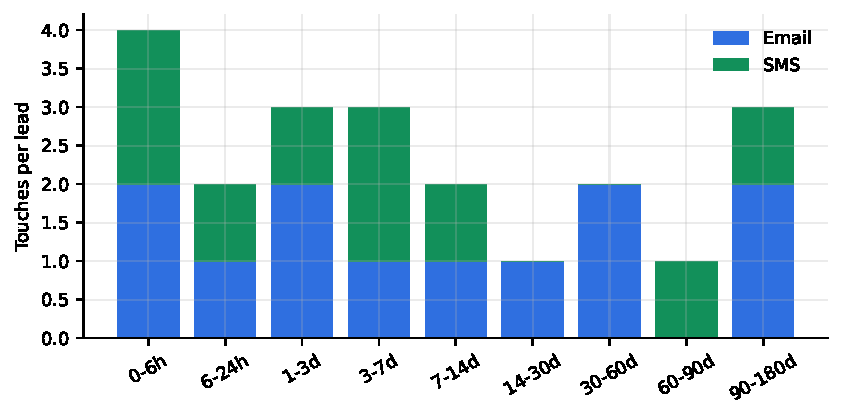
\includegraphics[width=0.8\linewidth]{fig/p3_buckets.pdf}\caption{Touches per lead by period.}\label{fig:bk}\end{figure}

\subsection{Response, fatigue and value}
In this segment 13.9\% of the cohort converts, 22\% unsubscribe and 64\% remain active at day 180 (Figure~\ref{fig:alive}). 61\% of incremental revenue arrives in the first 24 hours and 84\% within a week, which is the empirical motivation for the front-loaded design. Incremental revenue of 13,642\,\texteuro{} against sending costs of 3,834\,\texteuro{} (Figure~\ref{fig:cum}) gives net profit of 9,808\,\texteuro{} per 10{,}000 leads, a return of 2.6 per euro of cost, and lifts LTV per lead from 11.00\,\texteuro{} to 11.98\,\texteuro{}.
\begin{figure}[H]\centering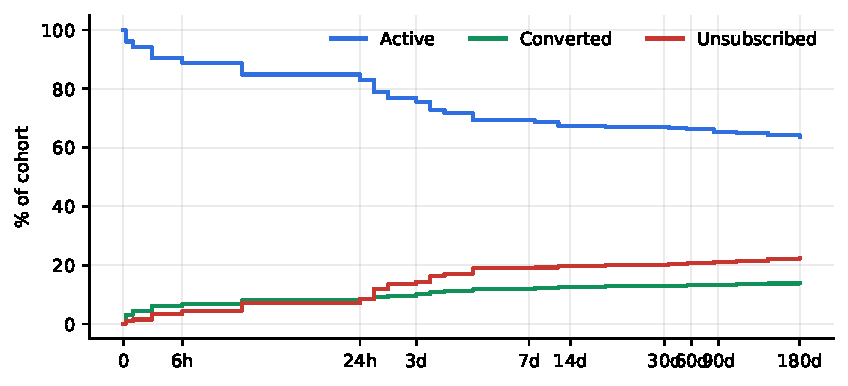
\includegraphics[width=0.8\linewidth]{fig/p3_alive.pdf}\caption{Share of the cohort active, converted and unsubscribed over time.}\label{fig:alive}\end{figure}

\begin{figure}[H]\centering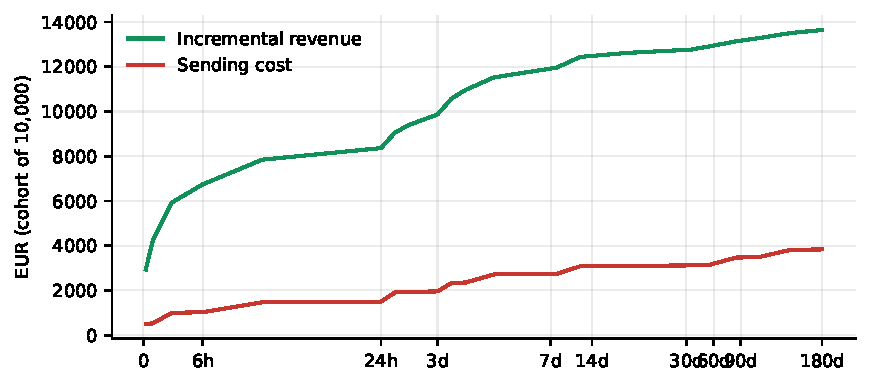
\includegraphics[width=0.8\linewidth]{fig/p3_cum.pdf}\caption{Cumulative incremental revenue and sending cost.}\label{fig:cum}\end{figure}

\subsection{All segments and alternative calendars}
Table~\ref{tab:res} reports results for every segment. The front-loaded calendar is profitable in four of six segments; the declined and cold-base segments lose money under these parameters, which indicates that they should receive fewer touches or a different offer rather than the same intensity.
\begin{table}[H]\centering\small\caption{Results per 10{,}000 leads: net profit (euros), return on cost, LTV per lead (euros), revenue share in the first 24 hours and share of the cohort that unsubscribes.}\label{tab:res}
\begin{tabular}{lrrrrr}\toprule Segment & Net profit & ROI & LTV/lead & First 24 h & Unsub.\\\midrule
Application submitted & 9,808 & 2.6 & 11.98 & 61\% & 22\%\\
First-step drop-off & 9,725 & 2.5 & 6.97 & 68\% & 18\%\\
Declined by all lenders & -185 & -0.1 & 1.98 & 46\% & 12\%\\
Payment-default flag & 646 & 0.2 & 3.06 & 53\% & 12\%\\
High-quality lead & 28,096 & 8.4 & 20.81 & 64\% & 17\%\\
Cold base & -581 & -0.2 & 0.94 & 35\% & 13\%\\
\bottomrule\end{tabular}\end{table}
We compare the designed calendar against (a) one email per week for 25 weeks and (b) an aggressive schedule of daily emails and SMS every other day for 30 days followed by weekly emails. Table~\ref{tab:strat} and Figure~\ref{fig:strat} show net profit. The front-loaded calendar has the highest net profit in one segment (first-step drop-off), beats the weekly email in three segments and the aggressive schedule in four, and is never the worst of the three. The aggressive schedule earns more in the two segments with the highest conversion value (applied: +2\%; high quality: +30\%) but loses between 43\% and 52\% of the cohort to unsubscribes, against 12\% to 22\% for the front-loaded calendar. The model assigns no cost to a lost contact beyond forgone conversions, so it is biased in favour of aggressive contact. The weekly email wins in the three lowest-value segments (declined, payment-default flag, cold base), where SMS and extra touches do not repay their cost.
\begin{table}[H]\centering\small\caption{Net profit (euros per 10{,}000 leads) of three calendars.}\label{tab:strat}
\begin{tabular}{lrrr}\toprule Segment & Front-loaded & Weekly email & Aggressive\\\midrule
Application submitted & 9,808 & 4,892 & 9,979\\
First-step drop-off & 9,725 & 5,295 & 8,573\\
Declined by all lenders & -185 & 932 & -1,358\\
Payment-default flag & 646 & 1,349 & -44\\
High-quality lead & 28,096 & 14,646 & 36,438\\
Cold base & -581 & 1,890 & -657\\
\bottomrule\end{tabular}\end{table}
\begin{figure}[H]\centering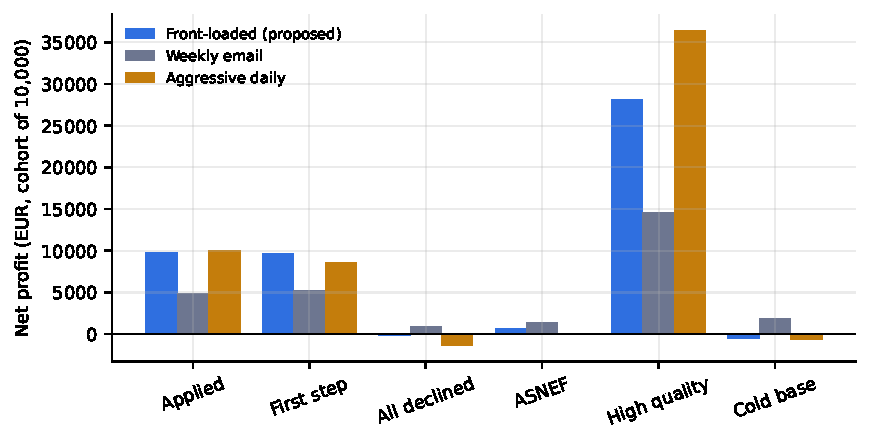
\includegraphics[width=0.85\linewidth]{fig/p3_strat.pdf}\caption{Net profit under three calendars in each segment.}\label{fig:strat}\end{figure}

\subsection{Sensitivity}
Figure~\ref{fig:sens} varies each assumption by $\pm25\%$ for the main segment. Base net profit is 9,808\,\texteuro{}. Response and conversion value are the most influential inputs (3,203\,\texteuro{} for $+25\%$ response), followed by incrementality; the unsubscribe rate matters less than expected over a six-month horizon, because most conversions occur early.
\begin{figure}[H]\centering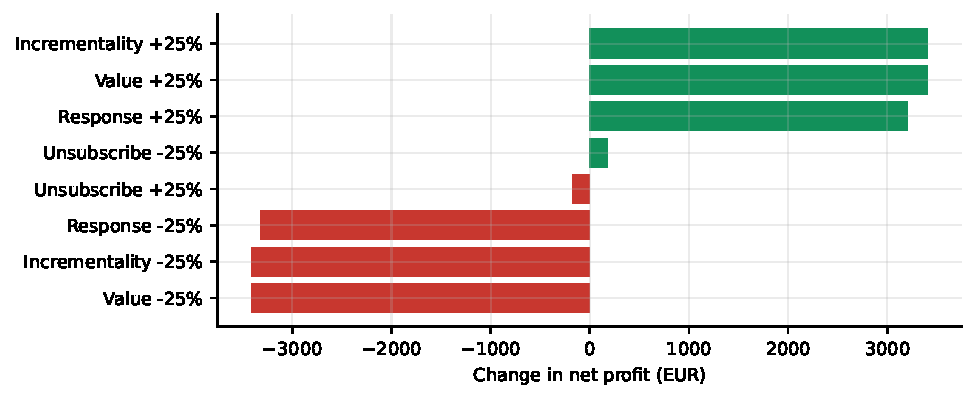
\includegraphics[width=0.8\linewidth]{fig/p3_sens.pdf}\caption{Sensitivity of net profit for the main segment.}\label{fig:sens}\end{figure}


\section{Validation design}
Every conclusion above depends on assumed parameters, so the calendar is a starting hypothesis. We recommend a holdout design \cite{kohavi}: randomly withhold a share of each segment (for example 10--20\%) from the flow; measure conversions per lead in treatment and holdout over the horizon, which gives $\iota$ directly; then test cadence variants (front-loaded against weekly) in randomised arms. Primary metric: incremental net profit per lead; guardrails: unsubscribe and spam-complaint rates. The sample needed to detect a difference in conversion rates $p_1,p_2$ is roughly $16\,\bar p(1-\bar p)/(p_1-p_2)^2$ per arm at 80\% power and 5\% significance, which for a difference of one point on a 5\% base is about 7{,}600 leads per arm.

\section{Limitations and compliance}
Parameters are hypotheses and the response model is stylised: no channel interaction, no time-of-day effect, no message content effect, and response is independent across leads. Commercial email and SMS require valid consent and an easy way to opt out; contact outside reasonable hours should be avoided, and regional rules on data protection and electronic communications apply. The planner stops at 180 days, but retaining contact data for longer has its own legal basis requirements.

\section{Conclusion}
A planner built on a small response model produces a transparent, editable calendar that front-loads contacts and expires leads at six months. The front-loaded design is a robust compromise rather than a uniform winner: more intense contact pays only where conversion value is high, and less intense contact wins where it is low. These conclusions come from the model's structure (decay, fatigue, unit costs) and from hypothesised parameters, not from measured effects, so the right next step is a holdout experiment.

\begin{thebibliography}{9}
\bibitem{gupta} S.~Gupta, D.~Hanssens, B.~Hardie, W.~Kahn, V.~Kumar, N.~Lin, N.~Ravishanker, S.~Sriram. Modeling customer lifetime value. \emph{Journal of Service Research}, 9(2):139--155, 2006.
\bibitem{kohavi} R.~Kohavi, D.~Tang, Y.~Xu. \emph{Trustworthy Online Controlled Experiments}. Cambridge University Press, 2020.
\end{thebibliography}
\end{document}
